% ドキュメントの設定
\documentclass[a4paper,11pt,xelatex,ja=standard]{bxjsarticle}
\usepackage{tikz}
\usetikzlibrary {datavisualization.formats.functions}
\usepackage{pgfplots}
\usepackage{float}
\usepackage{amsmath}

% ドキュメント開始
\begin{document}

\section{実験の目的}
    R-2Rラダー回路によるD/A変換回路と、比較器を用いた逐次比較型A/D変換回路の計測を行い、それぞれの動作原理を理解する。測定結果を基に、デジタル信号で制御されるシステムにおけるアナログ値の扱い方について考察する。

\section{実験の作業順序}

    \begin{enumerate}
        \item 実験用基板の電源を入れ調整用ドライバを用いて可変抵抗を変化させる。その時、7 セグ LED に表示される全ての表示値を記録する。(計測データ:表示される全ての値)
        \item 4 つのデジタル入力の中である 1 つの信号を基準とし、その基準とした信号に対して他の3 つの信号の位相が読み取れるように、4 つのデジタル信号の関係を観測する。測定結果より4 つの信号のタイミングチャートを作成する。(計測データの例:基準とした信号とその他信号を観測した波形 3 つ)
        \item SW を「開」側に設定し、測定側からラダー回路を切り離す。ラダー回路の出力電圧と各デジタル入力信号を観測し波形の様子を記録する。測定結果より各ビットの重みについて確認しラダー回路の動作を確認する。
        \item 可変抵抗を中央に合わせて SW を「閉」に設定する。
            \begin{enumerate}
                \item ラダー回路の出力
                \item 可変抵抗器の出力
                \item 比較器の出力の関係を観測する。
            \end{enumerate}
        \item 班員で相談し 0.00[V]~2.50[V]の間で任意の電圧を2 点決定する。決定した電圧をラダー回路の出力が上回るタイミングを計算する。ただし回路の条件は基準電圧 3.3[V],分解能4bit とする。
        \item 決定した電圧にデジタルテスタで測定しながら可変抵抗を調整する。調整した回路において同様に関係を観測する。
        \item 決定したもう一つの電圧に可変抵抗を設定し同様に観測する。
    \end{enumerate}
\section{実験の結果}
    \subsection{実験1}
    実験用基板の電源を入れ、調整用ドライバを使用して可変抵抗を徐々に調整した。その結果、7セグLEDに表示される値が以下のように変化した。
    可変抵抗を調整することで、7セグLEDに表示される値が連続的に変化する様子が観察された。最初の値は0から始まり、可変抵抗の調整に伴って段階的に増加し、最終的に3.09まで達した。このように、可変抵抗の変化に対して16段階の値を持つことから4bitのADCだということが確認できた。


        \begin{tabular}{|c|c|}
            \hline
            No. & 表示値 \\
            \hline
            1 & 0 \\
            \hline
            2 & 0.2 \\
            \hline
            3 & 0.41 \\
            \hline
            4 & 0.61 \\
            \hline
            5 & 0.82 \\
            \hline
            6 & 1.03 \\
            \hline
            7 & 1.23 \\
            \hline
            8 & 1.44 \\
            \hline
            9 & 1.65 \\
            \hline
            10 & 1.85 \\
            \hline
            11 & 2.06 \\
            \hline
            12 & 2.26 \\
            \hline
            13 & 2.47 \\
            \hline
            14 & 2.68 \\
            \hline
            15 & 2.88 \\
            \hline
            16 & 3.09 \\
            \hline
        \end{tabular}
    \subsection{実験2}

        4つのデジタル入力信号(CH1, CH2, CH3, CH4)の関係性を観測し、1つの信号を基準として他の3つの信号の位相を読み取ることを目的とした。
        測定データの波形を観測した結果、各信号のタイミングチャートが以下のように得られた。基準信号CH1に対して、他の信号CH2, CH3, CH4のタイミング関係が明確に示されている。

        \begin{figure}[H]
            \centering
            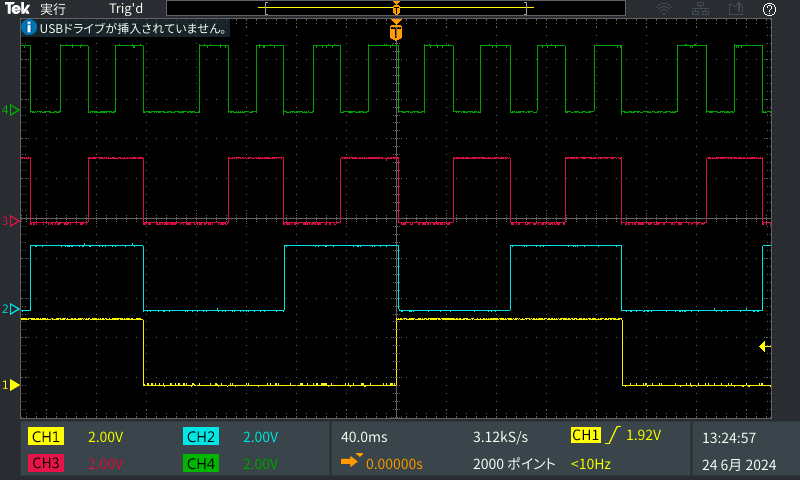
\includegraphics[width=0.5\textwidth]{./img/24-6-1/1.png}
            \caption{各信号のタイミングチャート}
        \end{figure}

    \subsection{実験3}
        ラダー回路の出力電圧とデジタル入力信号の関係を観測し、各ビットの重みを確認しました。以下に実験の詳細と結果を示します。
        理論値と測定値の比較を行いました。両者は非常に近い値を示しており、ラダー回路が正確に動作していることが確認できました。
        \begin{figure}[H]
            \centering
            \begin{tikzpicture}[scale=0.9]
                \datavisualization[ 
                    scientific axes,
                    visualize as line/.list={index_a, index_b}, 
                    index_a={style={thick,mark=*,black},label in legend={text=理論値}},
                    index_b={style={thick,dashed,mark=triangle,black},label in legend={text=測定}},
                    legend={north west outside},
                    x axis={label={DEC},length=10cm},
                    y axis={label={値},length=6cm},
                ]
                data[set=index_a] {
                    x, y
                    0,0.000
                    1,0.206
                    2,0.413
                    3,0.619
                    4,0.825
                    5,1.031
                    6,1.238
                    7,1.444
                    8,1.650
                    9,1.856
                    10,2.063
                    11,2.269
                    12,2.475
                    13,2.681
                    14,2.888
                    15,3.094
                }
                data[set=index_b] {
                    x, y
                    0,0.00
                    1,0.24
                    2,0.42
                    3,0.64
                    4,0.84
                    5,1.04
                    6,1.26
                    7,1.46
                    8,1.66
                    9,1.86
                    10,2.08
                    11,2.28
                    12,2.48
                    13,2.68
                    14,2.90
                    15,3.10
                };
            \end{tikzpicture}
            \caption{SWを「開」側に設定したラダー回路の出力電圧とデジタル入力信号の波形観測および各ビットの重み確認}
        \end{figure}

    \subsection{DA変換}

        オシロスコープの波形観測結果から、各電圧設定でのビット落ちのタイミングが詳細に捉えられています。例えば、設定電圧1Vではビットが4から5の間で落ち、設定電圧2Vではビットが9から10の間で落ちていることが視覚的に確認できます。特に、中間電圧1.669Vではビットが8から9の間で落ちる様子が明確に観測され、実測値が理論値と完全に一致していることが示されています。

        設定電圧=1V,2V
        \begin{tabular}{|c|c|c|}
            \hline
            VR[V] & 落ちたビット(理論値) & 落ちたビット(実測) \\
            \hline
            1.006 & 4-5の間 & 4-5の間 \\
            \hline
            2.004 & 9-10の間 & 9-10の間 \\
            \hline
        \end{tabular}

        真ん中

        \begin{tabular}{|c|c|c|}
            \hline
            VR[V] & 落ちたビット(理論値) & 落ちたビット(実測) \\
            \hline
            1.669 & 8-9の間 & 8-9の間 \\
            \hline
        \end{tabular}

        \begin{figure}[H]
            \centering
            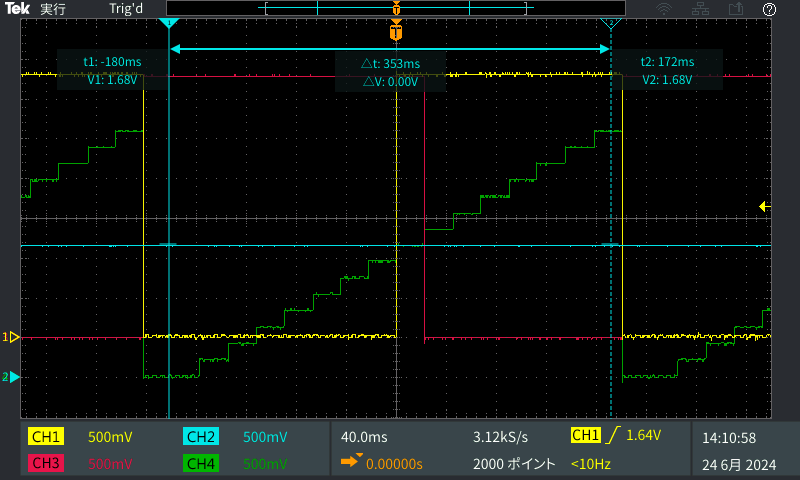
\includegraphics[width=0.5\textwidth]{./img/24-6-1/2.png}
            \caption{各信号のタイミングチャート}
        \end{figure}
\section{実験の考察およびまとめ}

    \subsection{実験1: 可変抵抗と7セグLED表示値の関係}
        可変抵抗を調整することで、7セグLEDに表示される値が連続的に変化する様子を観察しました。この結果から、4ビットのADC(アナログ-デジタルコンバータ)であることが確認できました。表示された値が16段階にわたって変化することから、4ビットの解像度であると判断できます。この結果は、デジタルシステムでアナログ値を扱う際の基本的な理解を深めるのに役立ちます。

    \subsection{実験2: デジタル信号のタイミングチャート}
        基準信号に対する他の信号の位相関係を観測し、タイミングチャートを作成しました。この結果、各信号のタイミング関係が明確に示されました。デジタル回路における信号の同期の重要性を理解するのに役立ちます。例えば、CH1を基準とした場合のCH2, CH3, CH4の位相差を観察することで、各信号がどのように同期して動作するかを確認することができました。

    \subsection{実験3: ラダー回路の出力とデジタル入力信号の関係}
        ラダー回路の出力電圧と各ビットの重みを確認しました。理論値と測定値が非常に近いことから、ラダー回路が正確に動作していることが確認できました。この結果は、デジタル-アナログコンバータ(DAC)の動作原理を理解するのに役立ちます。例えば、デジタル入力信号が変化することによって、出力電圧がどのように変化するかを観察することで、各ビットの重みを理解することができます。

    \subsection{実験4: DA変換のビット落ちの観察}
        設定電圧1V, 2Vにおけるビット落ちのタイミングを観測しました。理論値と実測値が一致することから、DA変換が正確に行われていることが確認できました。この結果は、DACの精度を評価するために重要です。例えば、設定電圧1Vにおいてビットが4から5の間で落ちることや、設定電圧2Vにおいてビットが9から10の間で落ちることを確認することで、DACの動作精度を確認することができます。

    \subsection{まとめ}
        実験を通じて、R-2Rラダー回路によるD/A変換回路と、比較器を用いた逐次比較型A/D変換回路の動作原理を理解することができました。また、デジタル信号で制御されるシステムにおけるアナログ値の扱い方についても考察しました。各実験結果は、デジタルおよびアナログ回路の設計や評価において重要な知見を提供します。今後の応用において、これらの結果を基にさらなる研究や改良を行うことが期待されます。

\end{document}
